\doublespacing
\setlength{\parindent}{1cm}

The research field of music information retrieval (MIR) has been evolving rapidly. Taken broadly, it covers the area of musicology, digital signal processing, machine learning, information retrieval and library science. As digital music service platforms such as iTunes, Spotify and Pandora have grown, so has been the need for MIR tools which to date has been largely written by programmers as scripts using C++ or MATLAB. In recent years, interest has grown within the MIR community in using (scientific) Python as a viable alternative [ref]. LibROSA is a python package for music and audio analysis. It provides the building blocks necessary to create music information retrieval systems. Here I provide a brief introduction to basic ideas and elements in libROSA as I have used this package in conducting bulk of the work in my thesis.
\par
In general, librosa’s functions tend to expose all relevant parameters to the caller. While this provides a great deal of flexibility to expert users, it can be overwhelming to novice users who simply need a consistent interface to process audio files. To satisfy both needs, they define a set of general conventions and standardized default parameter values shared across many functions.
\par
An audio signal is represented as a one-dimensional numpy array, denoted as y throughout librosa. Typically the signal y is accompanied by the sampling rate (denoted sr) which denotes the frequency (in Hz) at which values of y are sampled. The duration of a signal (d) can then be computed by dividing the number of samples (y) by the sampling rate (sr): \par
\begin{center}
  $ d = \frac{y}{sr} $
\end{center}

\begin{lstlisting}
# duration_seconds.py
from librosa import load
import os
# Getting all mp3 files of raga Bhairav from dataset
fileList = os.listdir("data/Hindustani/mp3/Bhairav")
# Creating dictionary to store number of samples and sampling rate
sampleDict = {}
# y is number of samples, sr is sampling rate of the audio file
for file in fileList:
  y, sr = load(file)
  sampleDict[file].append(y)
  sampleDict[file].append(sr)
  # calculating signal duration
  duration = y / sr
  sampleDict[file].append(duration)
\end{lstlisting}

By default, when loading stereo audio files, the librosa.load() function down mixes to mono by averaging left- and right-channels, and then resamples the monophonic signal to the default rate $ sr=22050Hz $. Most audio analysis methods operate not at the native sampling rate of the signal, but over small frames of the signal which are spaced by a hop length (in samples). The default frame and hop lengths are set to 2048 and 512 samples, respectively. At the default sampling rate of 22050 Hz, this corresponds to overlapping frames of approximately 93ms spaced by 23ms. Frames are centered by default, so frame index t corresponds to the slice:

\begin{lstlisting}
  y[(t*hop_length - frame_length/2):(t*hop_length+frame_length/2)]
\end{lstlisting}

where boundary conditions are handled by reflection padding the input signal y. For analyses that do not use fixed-width frames (such as the constant-Q transform), the default hop length of 512 is retained to facilitate alignment of results.

\par

The majority of feature analyses implemented by librosa produce two-dimensional outputs stored as numpy.ndarray, e.g., S[f, t] might contain the energy within a particular frequency band f at frame index t. We follow the convention that the final dimension provides the index over time, e.g., S[:, 0],  S[:,1] access features at the first and second frames. Feature arrays are organized column-major (Fortran style) in memory, so that common access patterns benefit from cache locality. By default, all pitch-based analyses are assumed to be relative to a 12-bin equal-tempered chromatic scale with a reference tuning of A440 = 440.0 Hz. Pitch and pitch-class analyses are arranged such that the 0th bin corresponds to C for pitch class or C1 (32.7 Hz) for absolute pitch measurements.

\par
\begin{flushleft}
  \textbf{Core Functionality}
\end{flushleft}

The librosa.core submodule includes a range of commonly used functions. Broadly, core functionality falls into four categories: audio and time-series operations, spectrogram calculation, time and frequency conversion, and pitch operations [ref]. For convenience, all functions within the core submodule are aliased at the top level of the package hierarchy, e.g., ``librosa.core.load'' is aliased to ``librosa.load''.
\par
Audio and time-series operations include functions such as: reading audio from disk via the audioread package [ref], resampling a signal at a desired rate, stereo to mono conversion, time-domain bounded auto-correlation, and zero-crossing detection. Spectrogram operations include the short-time Fourier transform (stft), inverse STFT (istft), and instantaneous frequency spectrogram (ifgram) [Abe \space 95], which provide much of the core functionality for down-stream feature analysis. Additionally, an efficient constant-Q transform (cqt) implementation based upon the recursive down-sampling method of Schoerkhuber and Klapuri [ref] is provided, which produces logarithmically-spaced frequency representations suitable for pitch-based signal analysis. Finally, logamplitude provides a flexible and robust implementation of log-amplitude scaling, which can be used to avoid numerical underflow and set an adaptive noise floor when converting from linear amplitude. Since data may be represented in a variety of time or frequency units, a comprehensive set of convenience functions is provided to map between different time representations: seconds, frames, or samples; and frequency representations: hertz, constant-Q basis index, Fourier basis index, Mel basis index, MIDI note number, or note in scientific pitch notation. Finally, the core submodule provides functionality to estimate the dominant frequency of STFT bins via parabolic interpolation (piptrack) [Smith \space 11], and estimation of tuning deviation (incents) from the frequency reference A440. These functions allow pitch-based analyses (e.g., cqt) to dynamically adapt filter banks to match the global tuning offset of a particular audio signal.

\par
\begin{flushleft}
  \textbf{Spectral Features}
\end{flushleft}

Spectral representations are the distributions of energy over a set of frequencies which form the basis of many analysis techniques in MIR and digital signal processing in general. Librosa implements a variety of spectral representations, most of which are based upon the short \space time Fourier transform. The Mel frequency scale is commonly used to represent audio signals, as it provides a rough model of human frequency perception [ref]. Both a Mel-scale spectrogram and the commonly used Mel-frequency Cepstral Coefficients (MFCC) are provided. By default, Mel scales are defined to match the implementation provided by Slaney’s auditory toolbox [ref], but they can be made to match the Hidden Markov Model Toolkit (HTK). While Mel \space scaled representations are commonly used to capture timbral aspects of music, they provide poor resolution o pitches and pitch classes. Pitch class (or chroma) representations are often used to encode harmony while suppressing variations in octave height, loudness, or timbre. Two flexible chroma implementations are provided: one uses a fixed-window STFT analysis (chroma \_ stft) [ref] and the other uses variable-window constant-Q transform analysis (chroma\_cqt). An alternative representation of pitch and harmony can be obtained by the tonnetz function, which estimates tonal centroids as coordinates in a six-dimensional interval space using the method of Harte et \space al. [ref]. Figures 1,2,3, and 4 illustrate the difference between STFT, Mel spectrogram, chromagram, and Tonnetz representations.

\begin{flushleft}
  \textbf{Display}
\end{flushleft}

The display module provides simple interfaces to visually render audio data through matplotlib [ref]. The first function, display.waveplot simply renders the amplitude envelope of an audio signal y using matplotlib’s fill\_between function. For efficiency purposes, the signal is dynamically down-sampled.
\par
Mono signals are rendered symmetrically about the horizontal axis; stereo signals are rendered with the left-channel’s amplitude above the axis and the right-channel’s below. An example of waveplot is depicted in Figure 5. The second function, display.specshow wraps matplotlib’s imshow function with default settings (origin and aspect) adapted to the expected defaults for visualizing spectrograms. Additionally, specshow dynamically selects appropriate colormaps (binary, sequential, or diverging) from the data type and range [ref]. Finally, specshow provides a variety of acoustically relevant axis labeling and scaling parameters. Examples of specshow output are displayed in Figures 1,2,3,4, and 5.

\begin{figure}
  \caption{Specshow Output for STFT Representation}
  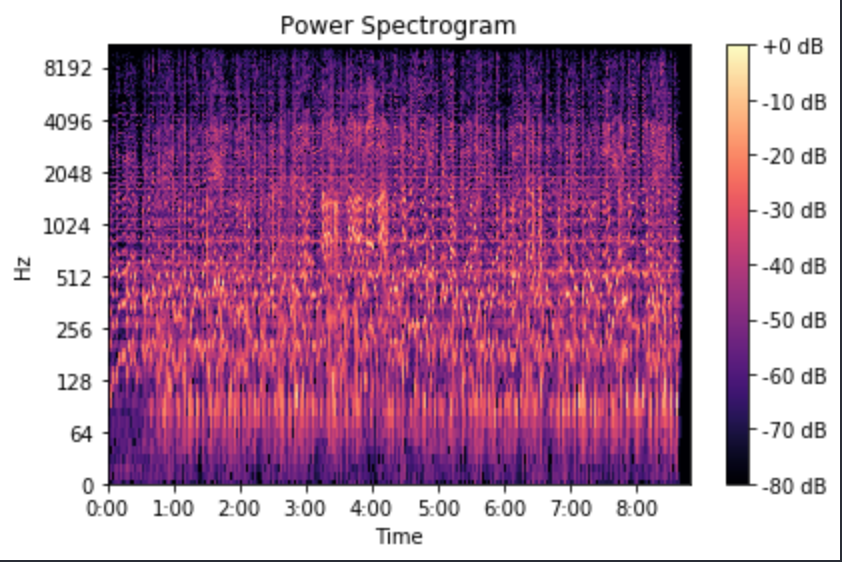
\includegraphics{stft-specgram.png}
\end{figure}
\begin{figure}
  \caption{Specshow Output for Mel Spectrogram Representation}
  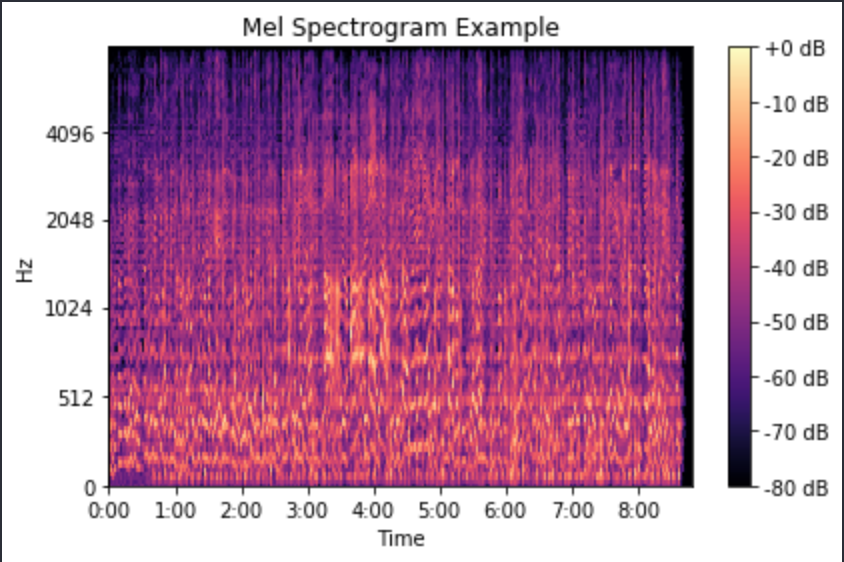
\includegraphics{mel-spectrogram.png}
\end{figure}
\begin{figure}
  \caption{Specshow Output for Chroma\_CQT Representation}
  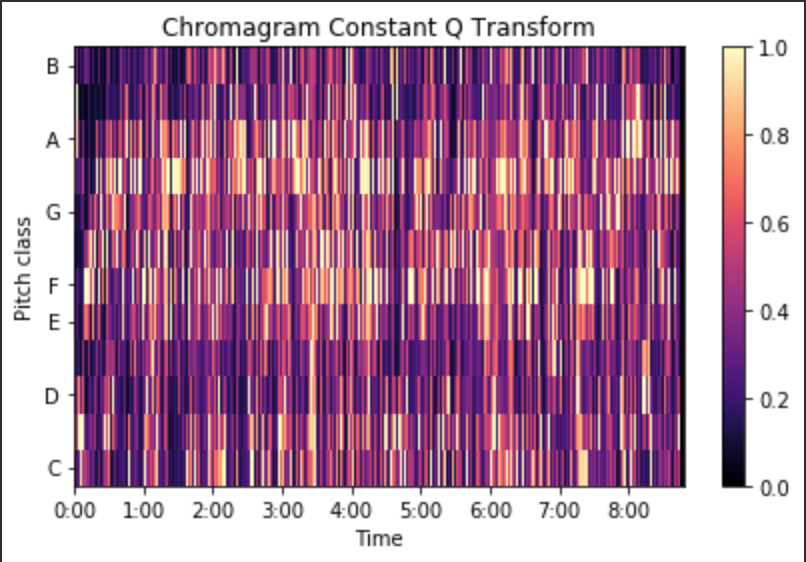
\includegraphics{chroma-cqt.png}
\end{figure}
\begin{figure}
  \caption{Specshow Output for Tonnetz Representation}
  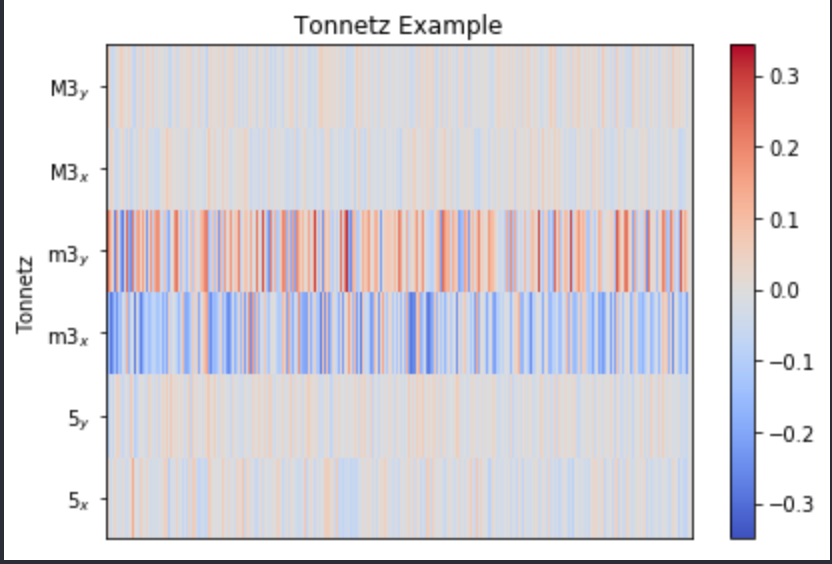
\includegraphics{tonnetz.png}
\end{figure}
\begin{figure}
  \caption{Specshow Output for Waveplot}
  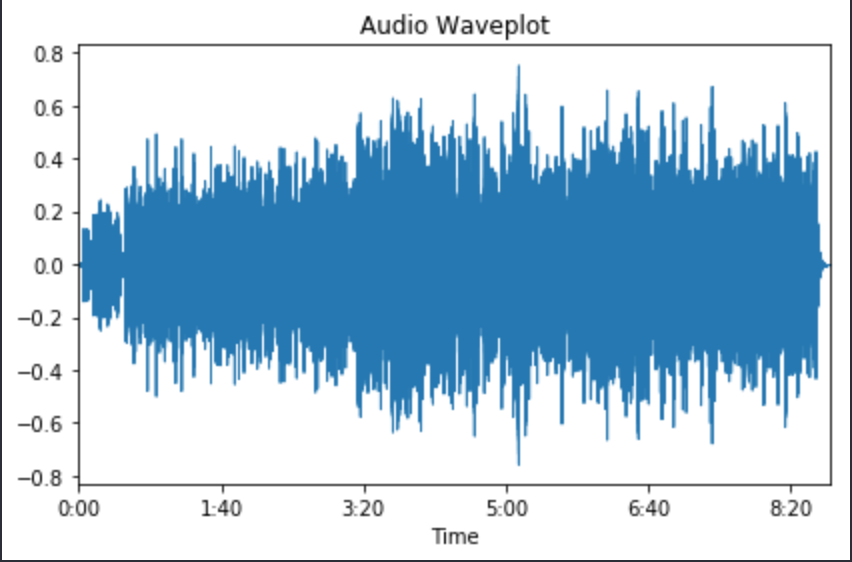
\includegraphics{waveplot.png} 
\end{figure}
